% -----------Incluir esto en caso necesario para que el capítulo comience siempre en página impar

%\newpage
%\thispagestyle{empty}
%\mbox{}
%---------------------------------------

\chapter{Introducción} 
\label{ch:chapter1}
\setlength{\parindent}{0cm}
\setlength{\parskip}{4mm}

\section{Motivación}\label{Motiv}

Un problema en la actualidad son las aguas contaminadas por sustancias de origen biológico, su importancia recae en la perdida de la biodiversidad o directamente implicar daños perjudiciales en la salud humana dado que las sustancias presentes en el agua pueden ser ingeridas por las especies marítimas que posteriormente son consumidas por los seres humanos.

Tomando en cuenta los avances tecnológicos de los sistemas robóticos de hoy en día, llegándose a considerar incluso como sistemas autónomos y programables capaces de realizar diversas tareas, se propone como objetivo de este proyecto el otorgar la capacidad de detectar y guiar a un conjunto de vehículos dispuestos sobre una superficie marítima hacia zonas de máxima concentración de sustancias toxicas.

Para ello, se deben tomar una serie de consideraciones:

\begin{enumerate}
	\item Los vehículos han de tener la capacidad de reunir datos del entorno, es decir, cada uno de ellos debe estar dotado de sensores para constantemente tomar medidas.
	\item Presentar una toma de decisiones para convertir dichos datos en acciones.
	\item La ejecución de la decisión tomada a través de su efector final.
\end{enumerate}

Por ende, se requiere de la utilización de vehículos que se puedan desplazar de manera autónoma por superficies marítimas y que agrupen todas las características comentadas hasta el momento. Consecuentemente, estas condiciones la cumplen los USV (vehículo autónomo de superficie), preguntar acá como hacer referencias abajo.

\begin{figure}[htb]
\centering
\includegraphics[width=0.6\textwidth]{figures/USV.eps}
\caption{Ejemplo de USV [referencia bibliografica]} \label{fig:USV}
\end{figure}

Por otro lado, los agentes han de ser capaces de cumplir su rol asignado una vez dispuestos alrededor de la forma simétrica adoptada, dicha misión consiste en avanzar desde un punto cualquiera a uno de interés que puede ser descrito mediante las \textbf{curvas de nivel}, en donde el punto de máximo valor se le puede atribuir el nombre de fuente. 

Otro aspecto fundamental es el como estos vehículos son capaces de detectar exactamente el punto de origen de máxima concentración o de coordinarse para ejercer el desplazamiento en torno a una superficie en concreta. Estos dos problemas que surgen se pueden resolver dotando a un grupo de robots la capacidad de coordinarse y colaborar para determinar dicha zona de máxima concentración para posteriormente desplazarse hacia ella, además deberá ser capaz de mantener una formación simétrica. Entre otras palabras, se requiere aplicar al caso un enjambre robótico más concretamente uno de tipo multiagente.

Cabe añadir que el punto de máxima concentración en la superficie sobre la que se desplazan los vehículos se puede definir mediante las curvas de nivel, además su variación va a estar estrictamente ligada con la distancia a la que este el centro de la formación con respecto al punto máximo, es decir, la intensidad radiada desde el punto fuente es una señal proporcional al inverso de la distancia al cuadrado definiendo una función cuadrática. Dicho esto, para modelar el mapa sobre el que se mueven los vehículos se propone una función gaussiana dado que cumple ser cóncava y cuadrática.

\begin{figure}[htb]
  \begin{center}
    \subfigure[Función definida en 3D]{
        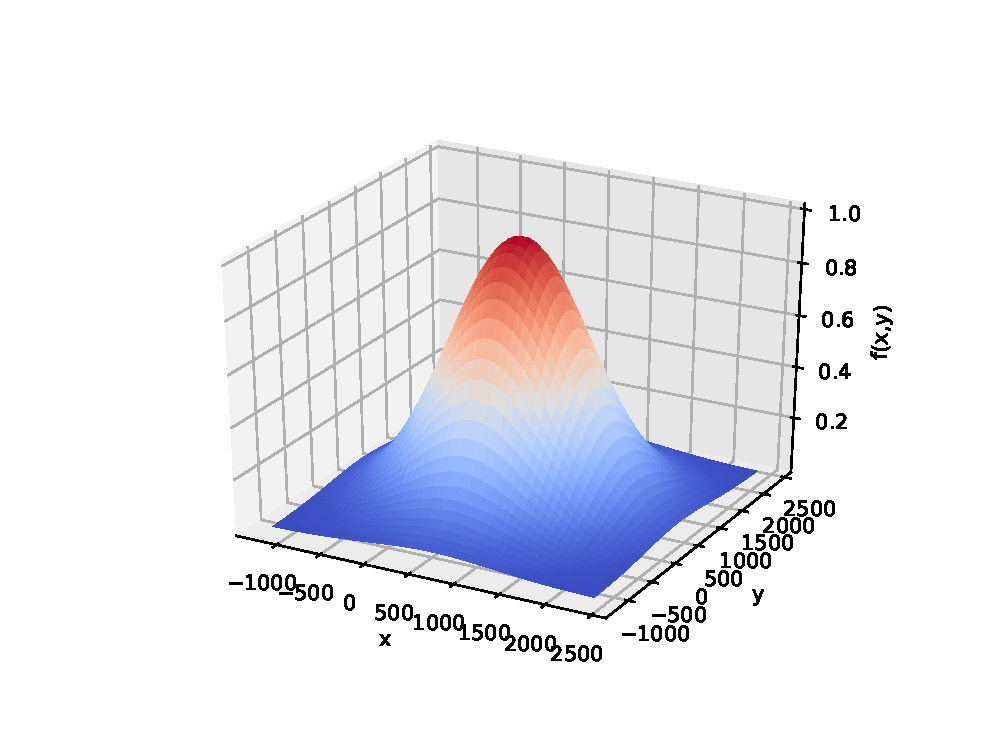
\includegraphics[width=0.45\textwidth]{figures/Gaussiana.eps}
        \label{Fgauss}}
    \subfigure[Curvas de nivel]{
        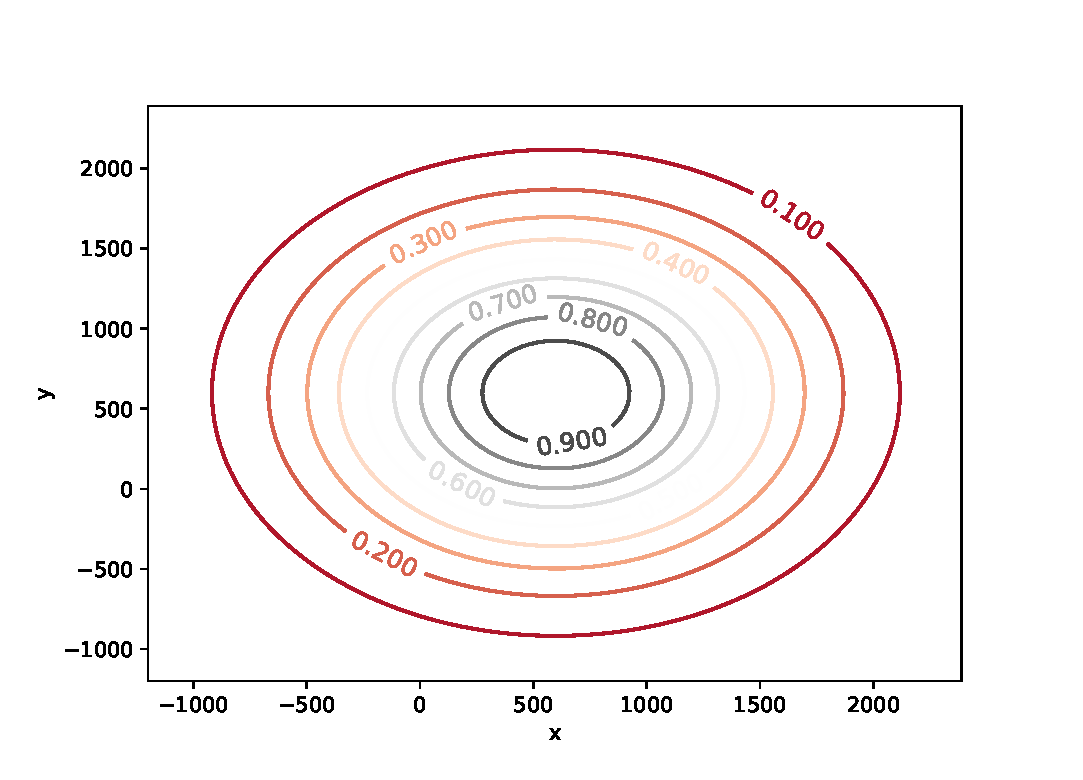
\includegraphics[width=0.45\textwidth]{figures/CurvasNivelGauss.eps}
        \label{CurvasGauss}}
    \caption{Representación de una función gaussiana}
    \label{FunGauss}
  \end{center}
\end{figure}

\section{Estado del arte}\label{Objetives}

La robótica de enjambre se basa en el comportamiento de los organismos sociales, en donde los individuos no han de tener un alto conocimiento para producir un comportamiento colectivo complejo, ni existir un líder que guía al resto para completar un objetivo, como en los bancos de peces, un panal de abejas o una bandada de pájaros.

Hoy en día, conforma un grupo de investigación muy activo por su versatilidad en diferentes ámbitos, tales como militar o industrial. En contraposición a tener un único robot realizando una labor compleja se tienen varios individuos simples para formar un comportamiento colectivo con el objetivo de realizar la misma tarea traduciéndose a su vez en una reducción de costes. Las características principales con las que se pueden definir los enjambres son:

\begin{enumerate}
	\item El número óptimo de agentes varía en función de la tarea asignada pudiendo ir desde tan pocos como una simple pareja hasta miles de unidades.
	\item Presenta gran \textbf{diversidad}, es decir, en ocasiones se mezclan robots simples o complejos, sistemas tripulados o no tripulados, e incluso con dominio cruzado.
	\item Para poder diferenciarlos de los sistemas multi-robots, en el que cada robot individualmente tiene una tarea asignada de antemano, los de tipo enjambre han de tener un \textbf{comportamiento colectivo} que involucre colaboración entre los propios agentes y estos con su entorno.
	\item Se necesita establecer una forma de comunicación entre los agentes para permitir el intercambio de información, esta puede ser implícita o explícita
	\item El hecho de que se puede definir su modo de operar no implica que se controle a cada robot individualmente, es decir, cada uno ellos han de poseer un comportamiento \textbf{autónomo} y \textbf{descentralizado}.
\end{enumerate}

Una aplicación al caso de los enjambres son los sistemas multiagentes que como bien su nombre indica, se basan en un grupo de dos o más agentes que interaccionan entre si para lograr un objetivo común en un mismo entorno. Dicha comunicación puede darse entre vecinos sin necesidad de recurrir a una entidad central, es decir, cada uno de ellos va a poseer un comportamiento autónomo y aun así conocer la existencia del resto.

Por tal motivo, la información va a estar distribuida en cada uno de los agentes con una rol distinto, además, se añade la posibilidad de fallo en cualquiera de ellos. Esto se traduce en un sistema más eficaz, flexible y fiable. 

\section{Objetivos}

Al principio de este capitulo se comentaron varias tareas que deben cumplirse para enfrentar el problema de la detección y posterior desplazamiento sobre superficie maritima hacia zonas dotadas de sustancias contaminantes. Este objetivo se logra mediante la cooperación de tres algoritmos.

El primero de ellos es un \textbf{algoritmo de búsqueda de fuentes} \cite{Estimacion_Gradiente} cuyo objetivo es detectar dicha zona de máxima concentración como un punto de inflexión de una función definida como cóncava, en donde, se asume que solo se tendrá una única fuente radiando y además que los agentes van a estar dispuestos en torno a una formación circular de manera simétrica para realizar las medidas correspondientes. 

Por otro lado, la necesidad del segundo algoritmo recae en la coordinación de los vehículos para adoptar una forma geométrica deseada más concretamente la formación circular previamente descrita es por ello que se va a utilizar un \textbf{algoritmo de control de formación circular} \cite{Control_Formacion}.

Además, el sistema en si debe tener la capacidad de dirigirse hacia la zona de interes por ello es que se va a hacer uso del \textbf{algoritmo de ascenso} en el que básicamente aprovechas funciones definidas como en la figura \ref{FunGauss} para desplazarte de forma ascendente, es decir, hacia un máximo.

Finalmente, se estudiará la eficacia de juntar estos tres algoritmos mediante diversos situaciones entre ellas destacan: la variación del número de vehículos, las posiciones desde donde empieces, el tamaño del radio de la formación o situaciones en las que se tienen varios focos radiando pero uno de ellos va a presentar la máxima concentración.

\section{Organización de la memoria}

Cuando termine describirlo mejor y mas organizado.

En el capítulo dos se dará una idea general del problema global haciendo uso de un diagrama de bloques, además, de describir brevemente diferentes aspectos necesarios para el desarrollo del problema. En el tercero se realiza la estimación previamente descrita. En el cuarto se aporta un algoritmo de control para la coordinación de los agentes de manera simétrica a lo largo de una formación circular. Finalmente, en el quinto y ultimo capítulo se dan los diferentes resultados obtenidos mediante la acción conjunta de ambos algoritmos.